\section{Shellcode}
\subsection{Definition}
Um den nächsten Teil besser zu verstehen, sollte vorher erklärt werden, was genau Shellcode ist, wofür er 
benutzt wird und was der Zusammenhang zur Assembler Programmiersprache ist. Shellcode ist definiert als eine 
Reihe von Anweisungen, die über einen Exploit injiziert und dann durch den Prozess ausgeführt werden.
Shellcode wird verwendet, um Register direkt zu manipulieren und die Funktionalität eines Programms auszunutzen. 
Es ist natürlich möglich, Shellcode in höheren Programmiersprachen zu schreiben, aber die effizienteste und fast 
ausschließlich benutzte Variante ist in der Sprache Assembly, die so maschinennah wie möglich ist, um genau steuern 
zu können was passiert und Speichergröße zu sparen. Meistens arbeitet man nämlich mit einer limitierten Speichergröße.
In der Computersicherheit bedeutet Shellcoding im wahrsten Sinne des Wortes das Schreiben von Code, der bei der
Ausführung eine Remote-Shell zurückgibt. Die Bedeutung von Shellcode hat sich weiterentwickelt und stellt nun jeden
Byte-Code dar, der in einen Exploit eingefügt wird, um eine gewünschte Aufgabe zu erfüllen. Da Shellcode in Assembly
geschrieben wird und die Sprache so maschinennah wie nur möglich ist, ist es außerdem noch wichtig mit welcher
Hardware und mit welchem Betriebssystem man diese schreibt. Es bestehen nämlich Unterschiede zwischen Linux
Shellcode und Windows Shellcode:  Bei Linux hat man direkten Zugriff auf das Interface und das Kernel, was bei
Windows leider nicht möglich ist. Im folgenden Beispiel wird ein Shellcode-Beispiel in der Sprache Assembly erläutert.
Die Idee hinter dem Beispiel ist es, zu zeigen, wie man mit einem Buffer Overflow Zugriff bekommen kann und dann den
vorbereiteten Shellcode injizieren kann, damit dieser privilegiert ausgeführt wird und somit Schaden am Ziel verursacht.

\subsection{Beispiel}
\begin{figure}[h]
    \centering
    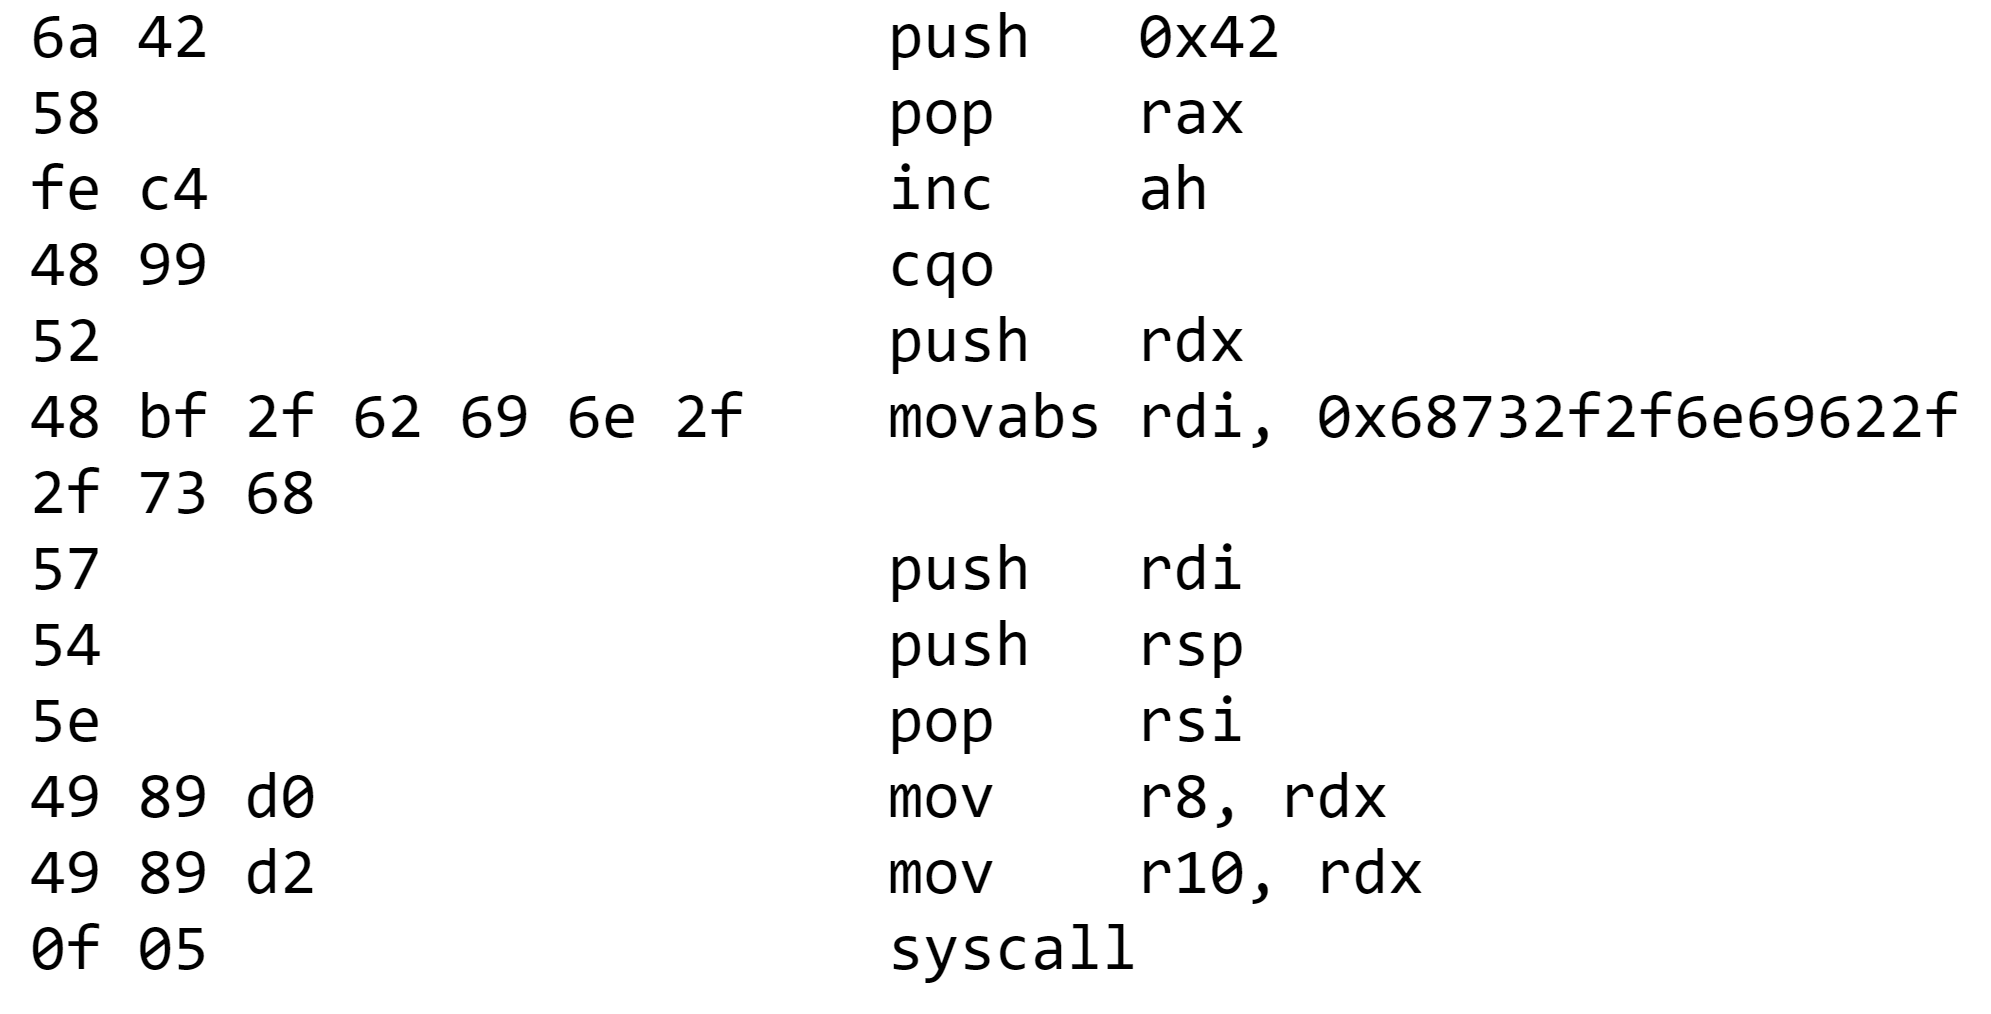
\includegraphics[width=0.9\textwidth,height=0.75\textheight,keepaspectratio]{images/shellstorm.png}
    \caption{Shellcode}
\end{figure}

%TODO: Einfügen aus DC
%Struktur:
%Der syscall wird abgeschickt, vorher müssen einige Werte gesetzt werden um execveat aufzurufen